\documentclass[titlepage=firstiscover, captions=tableheading, bibliography=totoc]{scrartcl}
\usepackage[autostyle=true,german=quotes]{csquotes}
\usepackage{scrhack}
\usepackage{caption}
\usepackage[aux]{rerunfilecheck}
\usepackage{subcaption}        
\usepackage{fontspec}
\usepackage[dvips]{graphicx}
\usepackage{floatflt,epsfig} 
    
\usepackage{polyglossia}
\setmainlanguage{german}

\usepackage[unicode]{hyperref}
\usepackage{bookmark}
\title{V27\\ Der Helium-Neon-Laser}
\author{
Miriam Simm\\
\texorpdfstring{\href{mailto:miriam.simm@tu-dortmund.de}{miriam.simm@tu-dortmund.de}\and}{,}
Katrin Bolsmann\\
\texorpdfstring{\href{mailto:katrin.bolsmann@tu-dortmund.de}{katrin.bolsmann@tu-dortmund.de}}{}
}
\date{Durchführung: 15.06.2020 \\ Abgabe: -.06.2020}
\usepackage{amsmath} 
\usepackage{amssymb} 
\usepackage{mathtools}
\usepackage[
    math-style=ISO,
    bold-style=ISO,
    sans-style=italic,
    nabla=upright,
    partial=upright,
]{unicode-math}
    
\setmathfont{Latin Modern Math}

\usepackage[
  locale=DE,
  separate-uncertainty=true, 
  per-mode=symbol-or-fraction,
]{siunitx}

\usepackage{multicol}
\setlength{\columnsep}{1pt} %space between columns 

\usepackage{booktabs}
\usepackage[x11names, table]{xcolor}
\usepackage{graphicx}
\usepackage{grffile}
\usepackage{xfrac}
\usepackage{xcolor}

\usepackage{float}
\floatplacement{figure}{h}
\floatplacement{table}{h}
\usepackage[
  section,
  below,
]{placeins}

\usepackage{expl3}
\usepackage{xparse}
\ExplSyntaxOn
\NewDocumentCommand \E {} {\symup{e}}
\ExplSyntaxOff

% Literaturverzeichnis
\usepackage[
  backend=biber,
]{biblatex}
% Quellendatenbank
\addbibresource{literatur.bib}

\usepackage[
  version=4,
  math-greek=default,
  text-greek=default,
]{mhchem}
 

\raggedcolumns

\begin{document}

\maketitle

\section{Auswertung}
\subsection{Bestimmung der maximalen magnetischen Flussdichte}
In Tabelle \ref{tab:atab1} sind die gemessenen Werte für die magnetische Flussdichte zu sehen. 

\FloatBarrier
\begin{table}[h]
    \centering
    \caption{Messwerte der Magnetischen Flussdichte $B(z)$.}
    \label{tab:atab1}
    \begin{tabular}{s s | s s}
        \toprule
        {z/mm} & {B/mT} & {z/mm} & {B/mT} \\
        \midrule
        100 & 116 & 114 & 396 \\
        101 & 150 & 115 & 395 \\
        102 & 184 & 116 & 393 \\
        103 & 215 & 117 & 386 \\
        104 & 252 & 118 & 376 \\
        105 & 289 & 119 & 364 \\
        106 & 314 & 120 & 345 \\
        107 & 339 & 121 & 323 \\
        108 & 357 & 122 & 293 \\
        109 & 372 & 123 & 262 \\
        110 & 382 & 124 & 227 \\
        111 & 390 & 125 & 190 \\
        112 & 394 & 126 & 153 \\
        113 & 396 & 127 & 125 \\
        \bottomrule
    \end{tabular}
\end{table}
\FloatBarrier
\noindent

Diese wurden in Abbildung \ref{fig:afig1} gegen $z$ aufgetragen und das Maximum bestimmt. 
Der Maximalwert der magnetischen Flussdichte entspricht dem Feld am Ort der Probe, somit wird für die nachfolgenen Rechnungen der Werte
\begin{equation}
	B = 396 \, \si{mT}
\end{equation}
verwendet.

\FloatBarrier
\begin{figure}[h]
    \centering
    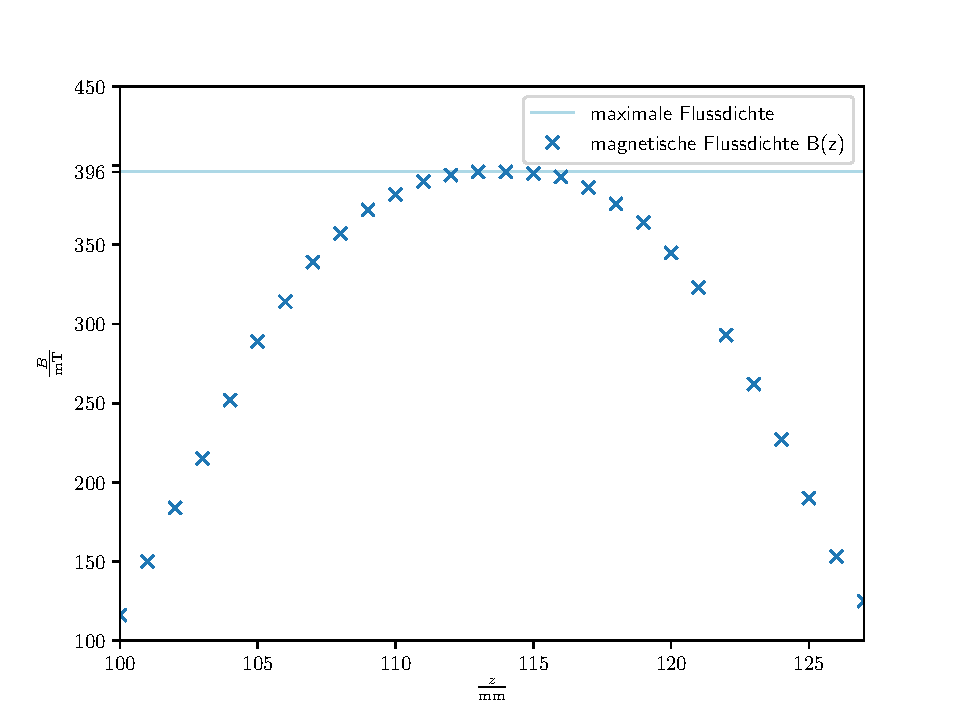
\includegraphics[width=\textwidth]{magnetfeld.pdf}
    \caption{Messwerte der Magnetische Flussdichte $B(z)$. Der Maximalwert liegt bei $B = 396\,\si{mT}$.}
    \label{fig:afig1}
\end{figure}
\FloatBarrier
\noindent


\subsection{Bestimmung der Rotationswinkel der Faraday Rotation}
Es wurden drei verschiedene Proben von Galliumarsenid untersucht. Hierbei handelt es sich um eine undotierte und zwei n-dotierte Proben, deren Eigenschaften in Tabelle \ref{tab:atab2} zu finden sind.

\FloatBarrier
\begin{table}[h]
    \centering
    \caption{Eigenschaften der untersuchten Galliumarsenidproben.}
    \label{tab:atab2}
    \begin{tabular}{l c c c}
        \toprule
        {} & {Probe 1} & {Probe 2} & {Probe 3} \\
        \midrule
        Dotierung N/$cm^{-3}$ & - & $1,2 \cdot 10^{18}$ & $2,8 \cdot 10^{18}$ \\
        Dicke d/mm & 5,11 & 1,36 & 1,296 \\
        \bottomrule
    \end{tabular}
\end{table}
\FloatBarrier
\noindent


Die Messwerte der Drehwinkel sind in Tabelle \ref{tab:atab3} aufgelistet. Hierbei handelt es sich bei $\theta_1$ und $\theta_2$ je um die Winkel die bei unterschiedlich gepolten Magnetfeld gemessen wurden.

\FloatBarrier
\begin{table}[h]
    \centering
    \caption{Messdaten für die Rotationswinkel für je zwei Polrichtungen des Magnetfeldes $B$, für 3 verschiedene Proben bei verschiedenen Wellenlängen.}
    \sisetup{table-format=2.1}
    \label{tab:atab3}
    \begin{tabular}{l c c c c c c}
        \toprule
        & \multicolumn{2}{c}{Probe 1} & \multicolumn{2}{c}{Probe 2} & \multicolumn{2}{c}{Probe 3} \\
        \cmidrule(lr){2-3}\cmidrule(lr){4-5}\cmidrule(lr){6-7}
        {$\lambda / \si{\micro\meter}$} & {$\theta_1$} & {$\theta_2$} & {$\theta_1$} & {$\theta_2$} & {$\theta_1$} & {$\theta_2$} \\
        \midrule

        1,06 & 143°50' & 167°00' & 148°20' & 158°00' & 150°10' & 159°30' \\
        1,29 & 148°00' & 164°00' & 150°00' & 157°20' & 150°35' & 157°20' \\
        1,45 & 148°20' & 160°15' & 146°35' & 154°50' & 150°10' & 159°00' \\
        1,72 & 151°00' & 160°00' & 149°40' & 156°15' & 149°20' & 161°10' \\
        1,96 & 157°30' & 164°40' & 250°35' & 161°50' & 154°25' & 164°30' \\
        2,156& 159°15' & 169°45' & 249°10' & 164°10' & 156°15' & 168°00' \\
        2,34 & 182°50' & 187°00' & 223°20' & 191°10' & 176°00' & 191°35' \\
        2,51 & 193°30' & 218°35' & 213°10' & 203°15' & 178°00' & 203°30' \\
        2,65 & 239°30' & 248°15' & 239°45' & 249°40' & 151°00' & 174°45' \\

        \bottomrule
    \end{tabular}
\end{table}
\FloatBarrier
\noindent

Für die nachfolgenden Rechnungen werden die Winkel, welche in Gradmaß angegeben sind, mittels der Formel
\begin{equation}
    1\, \symup{rad} = \frac{360°}{2\pi}
\end{equation}
in Bogenmaß umgerechnet. Hierbei ist zu beachten, dass die Gradmaß Skala auf $60$ skaliert ist und somit
\begin{equation*}
    1' = 0.1\bar{6}°
\end{equation*}
entspricht. Der auf die Probenlänge normierte Rotationswinkel der Polarisationsebene errechnet sich dann mittels der Formel
\begin{equation}
    \theta = \frac{1}{2\, L}(\theta_2 - \theta_1) \qquad .
\end{equation}
Damit die Längeneinheiten die gleiche Einheit besitzen, wurde $L$ hierzu in Mikrometer umgerechnet, da auch $\lambda$ diese Einheit hat.
In Tabelle \ref{tab:atab4} sind die umgerechneten und skalierten Werte des Rotationswinkels der einzelnen Proben zu finden. Diese Werte wurden anschließend für jede der Proben gegen $\lambda^2$ 
aufgetragen, wie in den Abbildungen \ref{fig:afig2}, \ref{fig:afig3} und \ref{fig:afig4} zu sehen ist.

\FloatBarrier
\begin{table}[h]
    \centering
    \caption{Die gemessenen Rotationswinkel der drei Proben je auf die Probendicke skaliert}
    \label{tab:atab4}
    \begin{tabular}{c c c}
        \toprule
        {$\theta_{\symup{Probe\,1}}/(10^{-5}\,\si{\micro\meter})$} & {$\theta_{\symup{Probe\,2}}/(10^{-5}\,\si{\micro\meter})$} & {$\theta_{\symup{Probe\,3}}/(10^{-5}\,\si{\micro\meter})$}\\
        \midrule
        4,03  & 6,20   &  6,28 \\
        2,73  & 4,70   &  4,55 \\
        2,03  & 5,29   &  5,95 \\
        1,54  & 4,22   &  7,97 \\
        1,22  & -56,94 &  6,79 \\
        1,79  & -54,54 &  7,91 \\
        0,71  & -20,64 &  8,42 \\
        4,28  & -6.37  &  4,94 \\
        1,49  & 6,37   &  10,83 \\
        \bottomrule 
    \end{tabular}
\end{table}
\FloatBarrier
\noindent
\FloatBarrier
\begin{figure}[h]
    \centering
    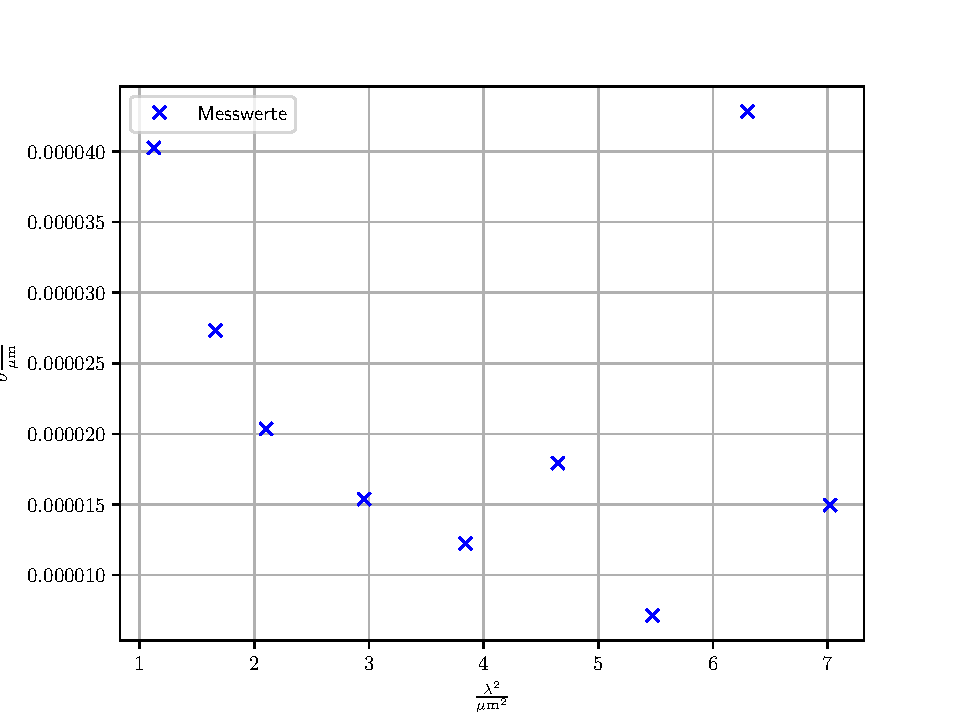
\includegraphics[width=1\textwidth]{Winkel_undotiert.pdf}
    \caption{Messwerte des Faraday-Roationswinkels der Messung mit der reinen Galliumarsenidprobe (Probe 1). Der Roationswinkel wurde hierzu auf die Länge der Probe $L = 5110 \si{\micro\meter}$ skaliert und gegen $\lambda ^2$ aufgetragen.}
    \label{fig:afig2}
\end{figure}
\FloatBarrier
\noindent

\noindent
\FloatBarrier
\begin{figure}[h]
    \centering
    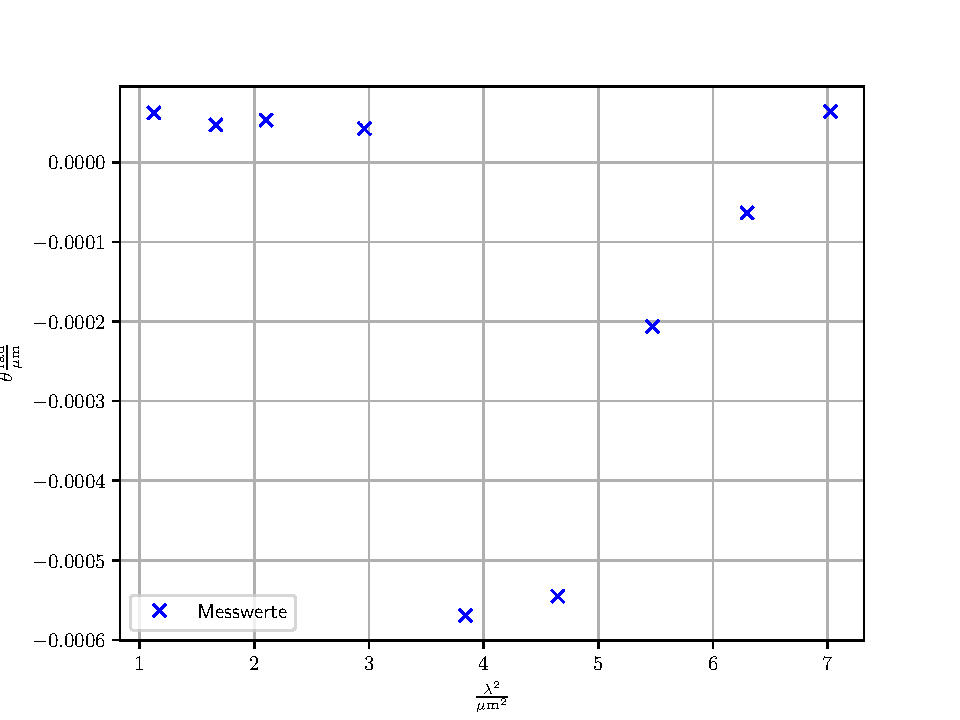
\includegraphics[width=1\textwidth]{Winkel_n-dotiert_1.pdf}
    \caption{Messwerte des Faraday-Roationswinkels der Messung mit der dotierten Galliumarsenidprobe (Probe 2) mit einer Dotierungsdichte von $N=1,2\cdot 10^{18}\, \si{cm}^{-3}$. Der Roationswinkel wurde hierzu auf die Länge der Probe $L = 1360 \si{\micro\meter}$ skaliert und gegen $\lambda ^2$ aufgetragen.}
    \label{fig:afig3}
\end{figure}
\FloatBarrier
\noindent

\noindent
\FloatBarrier
\begin{figure}[h]
    \centering
    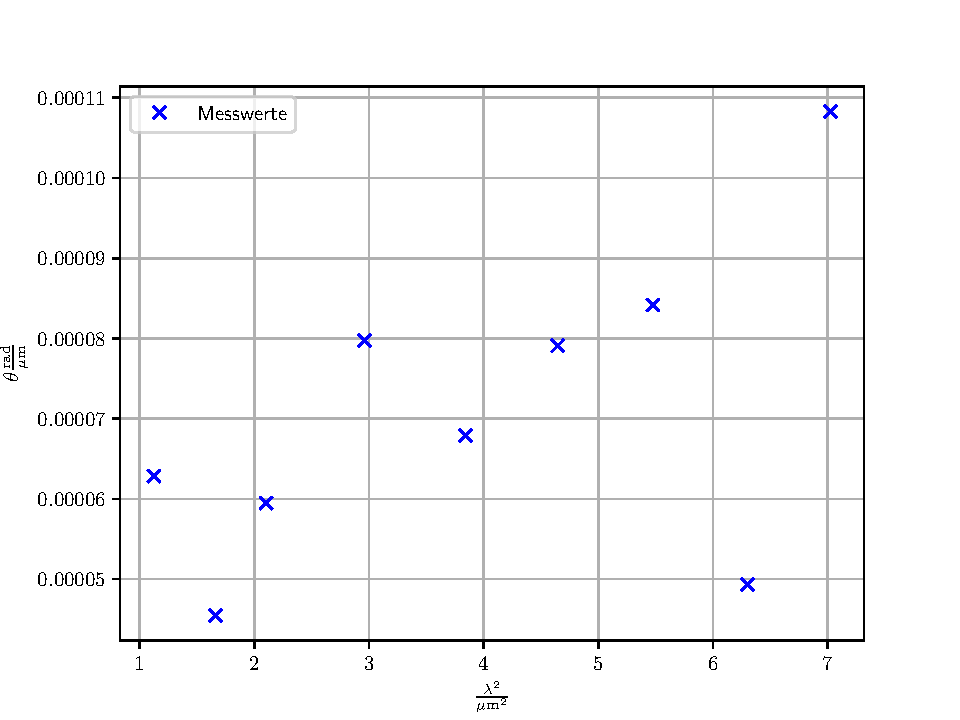
\includegraphics[width=1\textwidth]{Winkel_n-dotiert_2.pdf}
    \caption{Messwerte des Faraday-Roationswinkels der Messung mit der dotierten Galliumarsenidprobe (Probe 3) mit einer Dotierungsdichte von $N=2,8\cdot 10^{18}\, \si{cm}^{-3}$. Der Roationswinkel wurde hierzu auf die Länge der Probe $L = 1296 \si{\micro\meter}$ skaliert und gegen $\lambda ^2$ aufgetragen.}
    \label{fig:afig4}
\end{figure}
\FloatBarrier
\noindent

\subsection{Bestimmung der effektiven Masse der Elektronen in Galliumarsenid}
Um die effektive Masse der Elektronen in dem Halbleiter zu bestimmen, wird der Rotationswinkel der durch die Leitungselektronen hervorgerufen wird gemäß
\begin{equation}
    \theta_{\symup{frei}} = |\theta_{\symup{undotiert}}-\theta_{\symup{dotiert}}| \label{eq:diff}
\end{equation}
berechnet und anschließend gegen $\lambda^2$ aufgetragen, wie in Abbildungen \ref{fig:afig5} und \ref{fig:afig6} für beide dotierte Proben zu sehen ist. 

\noindent
\FloatBarrier
\begin{figure}[h]
    \centering
    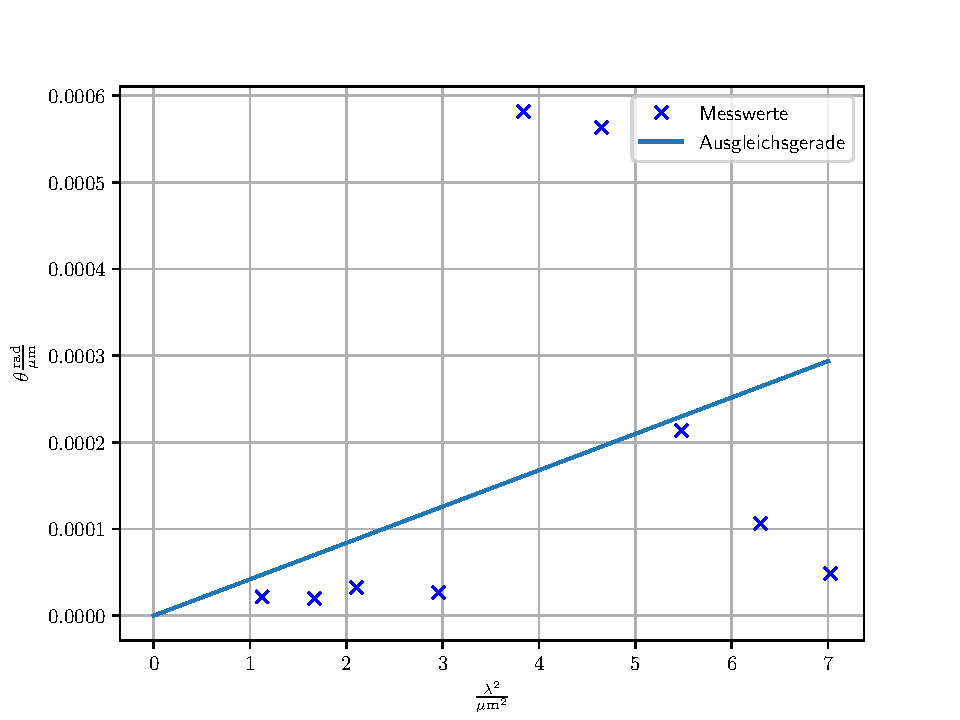
\includegraphics[width=1\textwidth]{Winkel_frei1.pdf}
    \caption{Der Rotationswinkel, welcher durch die Leitungselektronen hervorgerufen wird, aufgetragen gegen $\lambda^2$. Hierbei wurde $\theta_{\symup{frei}}$ aus dem Rotationswinkel der undotierten und der leicht dotierten Probe (Probe 2) gemäß \ref{eq:diff} berechnet.}
    \label{fig:afig5}
\end{figure}
\FloatBarrier
\noindent
\noindent
\FloatBarrier
\begin{figure}[h]
    \centering
    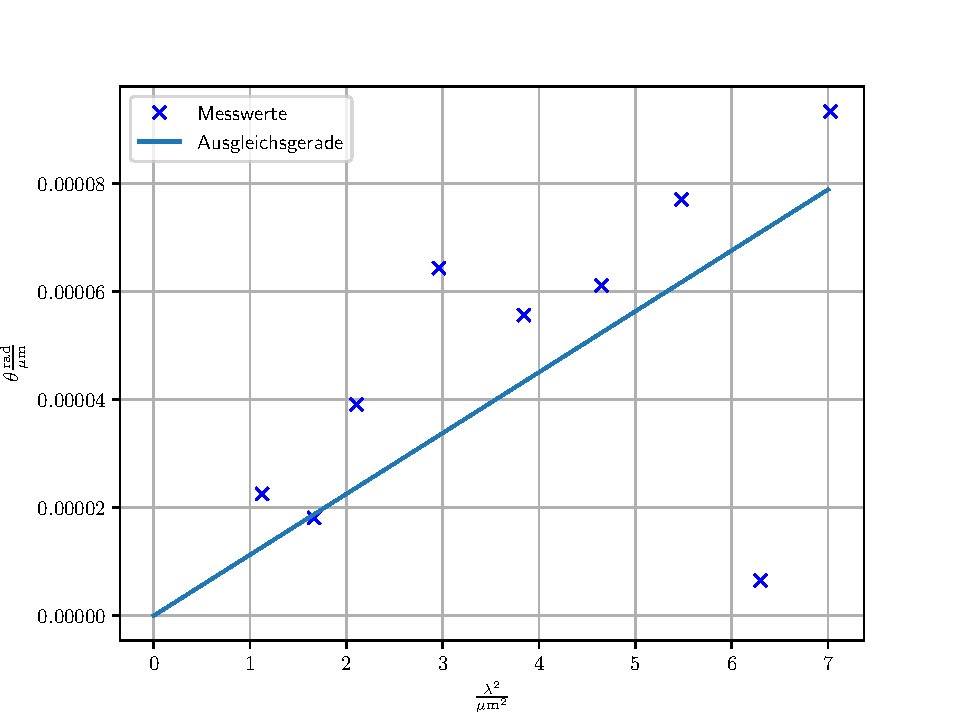
\includegraphics[width=1\textwidth]{Winkel_frei2.pdf}
    \caption{Der Rotationswinkel, welcher durch die Leitungselektronen hervorgerufen wird, aufgetragen gegen $\lambda^2$. Hierbei wurde $\theta_{\symup{frei}}$ aus dem Rotationswinkel der undotierten und der stärker dotierten Probe (Probe 3) gemäß \ref{eq:diff} berechnet.}
    \label{fig:afig6}
\end{figure}
\FloatBarrier
\noindent

Zur Ermittlung des Proportionalitätsfaktors zwischen $\theta_{\symup{frei}}$ und
$\lambda^2$ wird eine Ausgleichrechnung
\begin{equation*}
    \theta_{\symup{frei}}(\lambda^2) = a\cdot \lambda ^2
\end{equation*}
durchgeführt.
Für diese ergeben sich die Proportianilitätsfaktoren
\begin{align*}
    a_1 &= (4,196 \pm 0,003)10^{-5}\, \si{\micro\meter}^{-3}\\
    a_2 &= (1,127 \pm 0,004)10^{-5}\, \si{\micro\meter}^{-3} \qquad .
\end{align*}

Der Zusammenhang zwischen dem Rotationswinkel $\theta_{\symup{frei}}$ und der Wellenlänge $\lambda$ ist gemäß Formel \ref{eq:Winkel}
gegeben, woraus sich mittels Koeffizientenvergleich für den Proportionalitätsfaktor der Zusammenhang \ref{eq:Prop} ergibt. Durch Umstellen der Gleichung \ref{eq:Prop} ergibt
sich der Ausdruck, mit welchem die effektive Masse berechnet werden kann.
\begin{align}
   a &= \frac{e_0^3 \, N \, B}{8 \pi \epsilon_0 c^3 n (m^{*})^2}\\ \label{eq:Prop}
   \Leftrightarrow\qquad m &= \sqrt{\frac{e_0^3 \, N \, B}{8 \pi \epsilon_0 c^3 n a}}
\end{align}
ergibt. Zur Berechnung der effektiven Masse wird für den Brechungsindex der Literaturwert $n=3,857$ \cite[Quelle1] verwendet. Somit ergibt sich für die effektive Masse die beiden Werte
\begin{align*}
    m_1^{*} &= (0,02780 \pm 0.0001)\cdot m_e \\
    m_2^{*} &= (0.08192 \pm 0.0016)\cdot m_e \qquad .
\end{align*}

\section{Diskussion}
Wie zu erwarten, ist bei der Messung der Kraftflussdichte des Magnetfeldes ein kleines Plateau beim Maximalwert zu erkennen. Somit konnte der Wert für das Feld am Ort der Probe leicht bestimmt werden.

Die gemessenen Werte der Rotationswinkel des undotierten Leiters in Abbildung \ref{fig:afig2} zeigen nicht den nach \ref{eq:Winkel2} erwarteten $\sim \frac{1}{\lambda^2}$ Verlauf. Dies lässt sich womöglich durch Messfehler erklären.
Bei der Messung kam es bei einigen Wellenlängen zu dem Problem, dass der Nullabgleich sehr schwierig war. So kam es häufig bei kleineren Wellenlängen zu einer Übersteuerung des Selektivverstärkers. Ebenso ist aufgefallen, dass die Messung mit dem $1,72\,\si{\micro\meter}$
Plätchen besonders schwierig war, da dieses einige Mängel aufwies und somit schien es so, als würde mehr Licht durch dieses durchkommen, als es eigentlich sollte, da häufig eine Übersteuerung, bei minimaler Drehung des Glan-Thomson-Prismas auftrat.

Über den Verlauf der Messwerte in Abbildung \ref{fig:afig3} und \ref{fig:afig4} lässt sich vorerst keine Aussage machen, da hier der Einfluss aller Elektronen im Halbleiter eine Rolle spielt und somit keine genaue Aussage über die Abhängigkeit zur Wellenlänge $\lambda$ getroffen werden kann.
Jedoch sollte der Rotationswinkel des Faraday-Effekts, wenn der Einfluss der freien Elektronen isoliert wird, proportional zu $\lambda^2$ sein. Dieses Verhalten ist in den Abbildungen \ref{fig:afig5} und \ref{fig:afig6} nur begrenzt zu beobachten. Wobei die Ergebnisse der stärker dotierten Probe
bis auf einen Ausreißer, annähernd den erwarteten linearen Verlauf zeigen.

Das Ziel des Experiments war ist die effektive Masse der Leitungselektronen in Galliumarsenid zu bestimmen. Dieses erfolgte mit Hilfe der zuvor berechneten Proportionalitätsfaktoren zwischen Rotationswinkel $\theta_{\symup{frei}}$ und $\lambda^2$. Somit ergibt sich für die effektive Masse die beiden Werte
\begin{align*}
    m_1^{*} &= (0,02780 \pm 0.0010)\cdot m_e \\
    m_2^{*} &= (0.08192 \pm 0.0016)\cdot m_e \qquad .
\end{align*}
Verglichen mit dem Literaturwert für die effektive Masse der Leitungsbandelektronen im Halbleiter Galliumarsenid $m=0,063\, m_e$ \cite[Quelle2] weist der erste Wert eine Abweichung von circa $55\%$ auf, während der zweite Wert
mit einer Abweichung von circa $30\%$ dem Literaturwert deutlich näher kommt. Der Mittelwert der beiden Ergebnisse $\bar{m} = (0,05486 \pm 0.0005)\cdot m_e$ weist widerum eine Abweichung von nur $13\%$ auf. 

Zusammenfassend sind die Ergebnisse besser als der Verlauf der Messdaten zu Beginn vermuten lässt. Trotzdem sollte erwähnt werden, dass systematische Fehler dieses Experiment beinflusst haben. So war es zum Beispiel sehr schwerig die Apparatur genau zu justieren, was sich bereits dadurch zeigte, dass die Winkel bei dem der
Nullabgleich erreicht war keinen $90°$-periodischen Verlauf zeigten, sondern eher $100°$-periodischen waren. Außerdem ist der Brechungsindex $n$, welche für die Berechnung der effektiven Masse $m^{*}$ benötigt wurde, ebenfalls abhängig von der Wellenlänge. Dieser wurde in diesem Experiment aber als konstant angenommen.


\end{document}